\section{Summary of results and instructions to run your code.} \label{T7}

\paragraph{}To conclude, the above results shows us that both Hadoop and Spark gives no advantages when working with small datasets. However, if our datasets were a lot larger and the problem more complex, using Hadoop or Spark could have a significant performance impact over a plain Linux solution.

\paragraph{}The script needs to be run and should run correctly on any linux environment. However, it has only been tested on a Debian environment. To run our code, Python 3, Pip 3, Git and AWS CLI have to be installed on your machine. To make sure the script is executable, the command \verb|sudo chmod +x script.sh| must be executed. Our bash script can then be run as root with the command \verb|sudo ./script.sh|. Out git repository will then be automatically cloned and the \verb|run.sh| script will be executed, which will launch an interactive dialog.

\paragraph{}Alternatively, the script can be run manually. To do so, the repository must be cloned using this command:\\\verb|git clone https://github.com/JordMim/LOG8415E.git|. The script will then be located in the directory \verb|LOG8415E/tp2|. The script must be set as executable using the command \verb|sudo chmod +x run.sh|, and can then be run using the command \verb|sudo ./run.sh|.

\paragraph{}The deployment of our application on an AWS instance can be done using the first option of our run.sh script. This script guides the user while configuring AWS, then run a Python script that uses Boto3 for creating and configuring the Security Group and the Instance.

\paragraph{}To simplify the deployment on our AWS Instance, we decided to create a Docker image on which every dependencies are installed. By user a user\_data script, we automatically install Docker on the Instance and run a container based on this Docker image. This Docker image is based on Ubuntu 20.04 and contains Java 11, Hadoop 3.3.4, Python 3, PySpark 3.3.1. It also contain all the datasets. This all-in-one image gives the user the access over all the functionality through a REST API that respond to the port 80.

\paragraph{}More infos on the usage of the script is provided in the \href{https://github.com/JordMim/LOG8415E/blob/main/tp2/README.md}{\textbf{\emph{README.md}}} file of our repository.

\paragraph{}For each step of the script, the normal output should look like these:

\begin{center}
    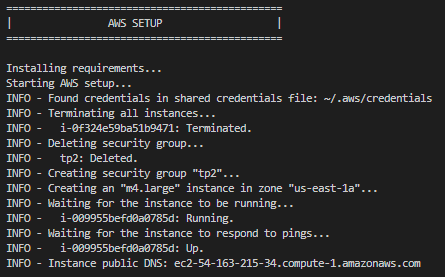
\includegraphics[width=14cm]{Resources/setup.png}\\
    \emph{Figure 7.1 - Output of the AWS Setup step}\\
    \hfill\\
    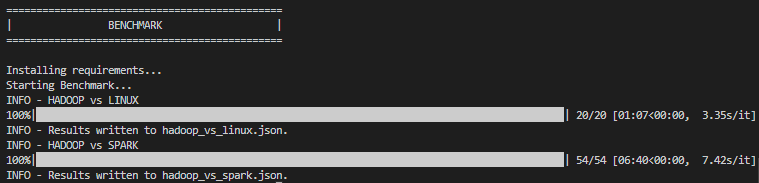
\includegraphics[width=14cm]{Resources/benchmark.png}\\
    \emph{Figure 7.2 - Output of the Benchmark step}\\
    \hfill\\
    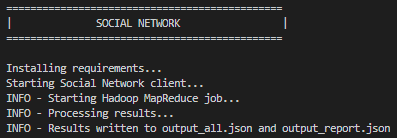
\includegraphics[width=14cm]{Resources/social.png}\\
    \emph{Figure 7.3 - Output of the Social Network step}\\
\end{center}
